% Compiles with REVTeX 4.2 when available (arXiv, full TeX Live); otherwise falls back to article.
\IfFileExists{revtex4-2.cls}{%
  \documentclass[aps,prd,preprint,superscriptaddress,nofootinbib,longbibliography]{revtex4-2}%
  \def\usingrevtex{1}%
}{%
  \documentclass[11pt]{article}%
  \usepackage[margin=1in]{geometry}%
  \usepackage[numbers,sort&compress]{natbib}%
}
\usepackage{amsmath,amssymb,amsthm}
\usepackage{graphicx}
\usepackage{longtable,booktabs,array,calc}

\usepackage[utf8]{inputenc}

\usepackage{microtype}
\usepackage{xcolor}
\usepackage[colorlinks=true,linkcolor=blue!50!black,citecolor=blue!50!black,urlcolor=blue!50!black]{hyperref}
\providecommand{\tightlist}{\setlength{\itemsep}{0pt}\setlength{\parskip}{0pt}}
\newcommand{\passthrough}[1]{#1}
\makeatletter
\def\fps@figure{htbp}
\makeatother
\setlength{\LTcapwidth}{\textwidth}
\ifdefined\usingrevtex\else
  \renewcommand{\thesection}{\Roman{section}}
  \renewcommand{\thesubsection}{\Alph{subsection}}
\fi

\begin{document}

\title{Causal Sets by Dynamical Densification:\\ Continuum Limit, Order-Only Rules, and Phase Interference}

\ifdefined\usingrevtex
  \author{Felix Xia}
  \email{felix@felixtw.tw}
  \affiliation{Independent researcher, Taiwan}
  \date{\today}
  \begin{abstract}
  We study a growth model for causal sets in which every new element is
inserted into the interior of the existing causal set, so that the
density of elements increases dynamically. The insertion rule is Lorentz
invariant: a child is placed at a small, Poisson-distributed proper-time
separation from a uniformly chosen parent, with a rapidity drawn from
the Haar measure \(\sinh^2\eta\,d\eta\), optionally damped by a
Maxwell--Jüttner factor \(e^{-\alpha\cosh\eta}\) whose rest frame is
read off the state. We use the model to address four open problems of
causal set theory.

\emph{Continuum limit.} The empirical measure of the growing set
converges almost surely for every \(\alpha\ge 0\), and every finite
induced-subposet density converges, so the process has a poset limit: a
uniform sprinkling of a conformally flat spacetime. For \(\alpha=0\) the
limit is explicit, \(a^4\propto t^2+(T-t)^2\).

\emph{Mesoscopic manifoldlikeness.} Exact second-moment recursions, an
eigenvalue criterion and martingale concentration give high-probability
versions of Madsen's conditions F2 (counting equals volume, uniformly
over all mesoscopic causal diamonds) and F3 (longest chain equals proper
time) for the conformal metric. Density clumping, a Pólya-urn effect, is
confined to wavelengths above \(8.0\)--\(9.1\) damping lengths.

\emph{Lorentz invariance versus locality.} Frame independence holds at
the 1--5\% resolution of intrinsic tests. Lorentz violation enters only
through the clumping excess and is negligible in the physical regime.

\emph{Rogue posets and quantum dynamics.} Order-only insertion rules
fail in three distinct ways, all traced to the light-cone nonlocality of
order-space neighbours, whose symmetric difference grows as \(N^{1/2}\)
in 2D and \(N^{0.8}\) in 4D. Attaching the phase
\(e^{i\beta S_{\rm BD}}\) to such histories, we prove a defect-gas
theorem: for \(M\) independent local defect sites with \(K\)
alternatives and uniformly distributed relative phases, the defect
amplitude grows as \(e^{M\,m(1+x_1+\dots+x_K)}\), where \(m\) is the
Mahler measure. The rate is zero for \(K=1\) and positive for
\(K\ge 2\), so multi-type local defects are not suppressed by
interference. Numerical checks support the uniform-phase hypothesis at
generic \(\beta\), additivity, the overlap correction and the absence of
double counting. The key analytic steps are machine-checked in Lean 4
with Mathlib.

  \end{abstract}
  \maketitle
\else
  \author{Felix Xia\\[2pt] {\small Independent researcher, Taiwan}\\ {\small\texttt{felix@felixtw.tw}}}
  \date{\today}
  \maketitle
  \begin{abstract}
  We study a growth model for causal sets in which every new element is
inserted into the interior of the existing causal set, so that the
density of elements increases dynamically. The insertion rule is Lorentz
invariant: a child is placed at a small, Poisson-distributed proper-time
separation from a uniformly chosen parent, with a rapidity drawn from
the Haar measure \(\sinh^2\eta\,d\eta\), optionally damped by a
Maxwell--Jüttner factor \(e^{-\alpha\cosh\eta}\) whose rest frame is
read off the state. We use the model to address four open problems of
causal set theory.

\emph{Continuum limit.} The empirical measure of the growing set
converges almost surely for every \(\alpha\ge 0\), and every finite
induced-subposet density converges, so the process has a poset limit: a
uniform sprinkling of a conformally flat spacetime. For \(\alpha=0\) the
limit is explicit, \(a^4\propto t^2+(T-t)^2\).

\emph{Mesoscopic manifoldlikeness.} Exact second-moment recursions, an
eigenvalue criterion and martingale concentration give high-probability
versions of Madsen's conditions F2 (counting equals volume, uniformly
over all mesoscopic causal diamonds) and F3 (longest chain equals proper
time) for the conformal metric. Density clumping, a Pólya-urn effect, is
confined to wavelengths above \(8.0\)--\(9.1\) damping lengths.

\emph{Lorentz invariance versus locality.} Frame independence holds at
the 1--5\% resolution of intrinsic tests. Lorentz violation enters only
through the clumping excess and is negligible in the physical regime.

\emph{Rogue posets and quantum dynamics.} Order-only insertion rules
fail in three distinct ways, all traced to the light-cone nonlocality of
order-space neighbours, whose symmetric difference grows as \(N^{1/2}\)
in 2D and \(N^{0.8}\) in 4D. Attaching the phase
\(e^{i\beta S_{\rm BD}}\) to such histories, we prove a defect-gas
theorem: for \(M\) independent local defect sites with \(K\)
alternatives and uniformly distributed relative phases, the defect
amplitude grows as \(e^{M\,m(1+x_1+\dots+x_K)}\), where \(m\) is the
Mahler measure. The rate is zero for \(K=1\) and positive for
\(K\ge 2\), so multi-type local defects are not suppressed by
interference. Numerical checks support the uniform-phase hypothesis at
generic \(\beta\), additivity, the overlap correction and the absence of
double counting. The key analytic steps are machine-checked in Lean 4
with Mathlib.

  \end{abstract}
\fi

\hypertarget{introduction}{%
\section{Introduction}\label{introduction}}

A causal set is a locally finite partial order whose
elements are spacetime atoms and whose order is the causal
relation \cite{BLMS87, Surya19}. The programme rests on a
kinematic fact and a dynamical hope. The fact is that a
Poisson sprinkling of a Lorentzian manifold produces a
causal set that is statistically Lorentz invariant
\cite{BHS09}. The hope is that some dynamics will make such
manifoldlike causal sets dominate. Between the fact and the
hope stand four well-known problems
\cite{Surya19, Carlip24}.

\begin{enumerate}
\def\labelenumi{\arabic{enumi}.}
\tightlist
\item
  \textbf{Rogue posets.} Almost all partial orders on \(N\)
  elements are three-layer Kleitman--Rothschild (KR) orders,
  about \(2^{N^2/4}\) of them \cite{KR75}. Any dynamics
  must overcome this entropy, and the entropy of every other
  non-manifold class.
\item
  \textbf{Quantum dynamics.} The natural candidate is a sum
  over causal sets weighted by \(e^{i\beta S_{\rm BD}}\),
  with \(S_{\rm BD}\) the Benincasa--Dowker action
  \cite{BD10, DG13} and Sorkin's quantum measure as the
  interpretive frame \cite{Sorkin94}. Layered orders, KR
  orders included, are known to be strongly suppressed by
  the phase \cite{LC18, CCS23, CCS24}. What survives is not
  known \cite{Carlip24}.
\item
  \textbf{Lorentz invariance versus locality.} Sprinkled
  causal sets are Lorentz invariant because their links
  reach arbitrarily far along the light cone. Rules that are
  local in any frame break Lorentz invariance; rules that
  are Lorentz invariant are nonlocal
  \cite{BHS09, Sorkin07}.
\item
  \textbf{Continuum limit.} It is not settled in what sense
  a growing causal set converges to a manifold. For
  classical sequential growth \cite{RS00} the
  order-theoretic limits are understood \cite{BGe10}. For
  growth that inserts elements into the past, even the
  choice of observables is contested \cite{BDZ21}.
\end{enumerate}

This paper studies one model against all four problems. Its
defining choice is \textbf{dynamical densification}: each
new element is inserted into the interior of the existing
set, at a small proper-time separation from a randomly
chosen parent, with uniformly random rapidity. Classical
sequential growth instead adds elements only to the future
boundary, so that birth order is a time order. Densification
has three structural advantages. A superposition of
independent Poisson sprinklings is again a Poisson
sprinkling, so a rule that inserts uniformly by volume keeps
every intermediate stage a Lorentz-invariant sprinkling. The
continuum limit is then simply the limit of increasing
density. And the growth index becomes a resolution scale
rather than a time, which removes the requirement that the
past be settled. The price is that inserting an element
correctly requires knowing its relation to elements far away
along the light cone. Much of what follows measures that
price.

We call the coordinate version of the rule the
\emph{replication model}. A child \(y\) of parent \(p\) is
placed at proper time \(\tau\) with \(\tau^4\propto E\),
\(E\sim{\rm Exp}(1)\) in units of one element per
discreteness volume, and at rapidity \(\eta\) drawn from the
Haar measure \(\sinh^2\eta\,d\eta\,d\Omega\) of the Lorentz
group, optionally damped by \(e^{-\alpha\cosh\eta}\) in a
rest frame estimated from the state. The parameter
\(\alpha\) is the ratio of the discreteness length to a
damping length \(L_H=\ell/\alpha\), which we identify
physically with the Hubble radius, so \(\alpha\sim10^{-61}\)
today.

\hypertarget{summary-of-results}{%
\subsection{Summary of results}\label{summary-of-results}}

\begin{longtable}[]{@{}
  >{\raggedright\arraybackslash}p{(\columnwidth - 4\tabcolsep) * \real{0.1667}}
  >{\raggedright\arraybackslash}p{(\columnwidth - 4\tabcolsep) * \real{0.6833}}
  >{\raggedright\arraybackslash}p{(\columnwidth - 4\tabcolsep) * \real{0.1500}}@{}}
\toprule\noalign{}
\begin{minipage}[b]{\linewidth}\raggedright
Problem
\end{minipage} & \begin{minipage}[b]{\linewidth}\raggedright
Result
\end{minipage} & \begin{minipage}[b]{\linewidth}\raggedright
Status
\end{minipage} \\
\midrule\noalign{}
\endhead
\bottomrule\noalign{}
\endlastfoot
Continuum limit & Empirical measure converges a.s. for all
\(\alpha\ge0\); all induced-subposet densities converge; the
poset limit is a uniform sprinkling of \((M,a^2\eta)\);
explicit for \(\alpha=0\) (Theorems 17--20, Sec. V) & Proof;
abstract layer in Lean \\
Mesoscopic manifoldlikeness & High-probability F2 uniformly
over all diamonds and F3 with exponential tails, for the
conformal metric; clumping only above \(8.0\)--\(9.1\,L_H\)
(Propositions 1--3, 7; Theorems 4D, 5D, 8--10, 13, 16;
Lemmas 6D, 11, 12; Sec. IV) & Proof plus numerics \\
Lorentz versus locality & Frame independence at 1--5\%;
violation only through the clumping excess,
\(\propto (H/M_{\rm Pl})^2\) in the physical regime (Sec.
III) & Numerics plus estimates \\
Rogue posets & Coordinate-model output passes all intrinsic
tests; order-only insertion rules fail in three classified
ways, traced to nearest-neighbour symmetric differences
\(\propto N^{1/2}\) (2D) and \(\propto N^{0.8}\) (4D) (Sec.
VI) & Numerics \\
Quantum dynamics & Defect-gas theorem: rate \(=\) Mahler
measure, \(0\) for \(K=1\) and \(>0\) for \(K\ge2\); KR
threshold reproduced; interactions raise the
\(\beta\)-averaged rate (Theorem 21, Sec. VII) & Proof; core
steps in Lean; numerics \\
\end{longtable}

The overall picture is a division of labour. The replication
model supplies a kinematics that is Lorentz invariant at the
discreteness scale and converges to a conformally flat
continuum. The intrinsic test battery and the poset-limit
theorems verify that output using the order alone. The
quantum phase cannot replace a well-behaved classical
measure: it suppresses defects whose action shifts are
concentrated enough to phase-lock, as for layered and KR
orders, but not the multi-type local defects that order-only
growth rules generate.

Three limitations should be stated at the outset. The
replication rule places children in background coordinates,
so it is not a purely order-theoretic dynamics; Section VI
explains why we believe no simple order-only rule can
replace it. The large-scale conformal factor is fixed by
boundary conditions, not by the dynamics (Sec. II C). And
Theorem 21 assumes uniformly distributed relative phases, a
hypothesis we test numerically rather than prove.

\hypertarget{the-replication-model}{%
\section{The replication
model}\label{the-replication-model}}

The replication model grows a causal set inside a fixed
region by repeatedly choosing a parent uniformly among the
existing elements and inserting one child near it. ``Near''
is defined invariantly: the child lies at a small proper
time from the parent, in a uniformly random direction on the
hyperboloid. All results in this section are numerical and
set up the theorems of Secs. IV and V.

\hypertarget{the-11-dimensional-rule}{%
\subsection{The 1+1-dimensional
rule}\label{the-11-dimensional-rule}}

In two dimensions write the displacement in light-cone
coordinates. The child of \(p\) is placed at
\((\Delta u,\Delta v)=(\sqrt{s}\,e^{\eta},\sqrt{s}\,e^{-\eta})\),
where \(s\) is the invariant interval volume, chosen so that
the parent--child diamond contains on average
\(c\,{\rm Exp}(1)\) elements, and \(\eta\) is uniform on the
allowed range (the 1+1 Haar measure is flat in rapidity).
Sprinkled causal sets gain about \(\ln 2\) links per element
when \(N\) doubles, because links extend along the light
cone \cite{BHS09}. The rule reproduces this. For \(N=1\)k,
2k, 4k and \(c=1\) the mean link count per element is
\(5.17\to5.95\to6.59\), against \(5.49\to6.18\to6.87\) for
sprinkling, and the interval abundances
\(N_1/N_0,N_2/N_0,N_3/N_0\) agree with sprinkling to
\(\pm0.02\) for \(c=1\)--\(3\). A rule that is local in a
spatial slice instead gives \(2.92\to3.05\to3.08\) links and
abundances \(0.96\)--\(0.97\): it is not manifoldlike.

A placement field test confirms frame independence. We apply
Sorkin's smeared d'Alembertian \(B_\epsilon\)
\cite{Sorkin07} (\(\epsilon=0.1\)) to plane waves of fixed
invariant wavenumber and varying rapidity \(b\). The
response ratio \(R(b)/R(0)\) for the densifying network
stays within \(1.02\)--\(1.06\) for \(|b|\le 2.5\), as for
Poisson sprinkling, at about 5\% precision. A variant that
replicates only the leaves of the genealogy (``replication
of the present'') retains a 15--30\% frame dependence that
does not shrink from \(N=6\)k to \(12\)k. The reason is that
the Lorentz group is non-compact: a single splitting can
only draw rapidities from a bounded range, so the genealogy
keeps a preferred frame. Inserting into the existing
interior lets the usable rapidity range grow with \(N\).

\hypertarget{the-31-dimensional-rule}{%
\subsection{The 3+1-dimensional
rule}\label{the-31-dimensional-rule}}

In four dimensions the child is placed at proper time and
rapidity

\[\tau=\ell\left(\frac{24E}{\pi}\right)^{1/4},\quad E\sim{\rm Exp}(1),\qquad p(\eta)\,d\eta\propto\sinh^2\!\eta\;e^{-\alpha(\cosh\eta-1)}\,d\eta ,\]

with \(\Delta t=\pm\tau\cosh\eta\),
\(|\Delta\mathbf{x}|=\tau\sinh\eta\) and a uniformly random
spatial direction. Here \((\pi/24)\tau^4\) is the volume of
the parent--child diamond, so \(E\) is its expected element
count in units of the discreteness density. The sign of
\(\Delta t\) is chosen with probability \(1/2\)
(time-symmetric insertion) and children falling outside the
region are redrawn.

Two features have no 1+1 analogue. First, insertion must be
time-symmetric. In 1+1 dimensions every insertion in rank
coordinates is a monotone reparametrisation of \(u\) and
\(v\), i.e.~a conformal map, and the infinite-dimensional
conformal group absorbs it. In 3+1 dimensions it does not;
future-only growth collapses toward the final boundary (1584
of 2000 elements in the last sixth of the time range).
Second, the Haar measure is not normalisable. Without
damping (\(\alpha=0\)) the median spatial step grows as
\(N^{1/4}\), i.e.~in proportion to the region size, and the
large-scale density is set by the boundary (the diamond tips
are over-dense by a factor \(2.4\)--\(3.2\), independent of
\(N\) from 2k to 32k).

The local structure is nevertheless Lorentz invariant. Our
order-only \emph{diamond test} selects parent--child pairs
whose interval contains \(60\pm10\%\) elements, measures the
Myrheim--Meyer dimension, links per element, longest chain
and \(N_1/N_0\) inside, and bins by the rapidity \(b\) of
the separation. For \(N=32\)k the change between
\(b\in[1.2,1.6)\) and \(b\in[0,0.4)\) is within one standard
error for Haar replication
(e.g.~\(\Delta d_{\rm MM}=+0.014\), \(0.9\) s.e.) and for
Poisson sprinkling, while a lattice control drifts by
\(12\)--\(15\) s.e.

\hypertarget{damping-the-state-determined-frame-and-what-replication-cannot-do}{%
\subsection{Damping, the state-determined frame, and what
replication cannot
do}\label{damping-the-state-determined-frame-and-what-replication-cannot-do}}

Damping by \(e^{-\alpha\cosh\eta}\) cures the boundary
pile-up at the cost of a frame \(u\) in which \(\cosh\eta\)
is measured. We define \(u\) from the state: \(u(p)\) is the
normalised sum of future unit vectors to the \(K\) related
elements of smallest interval volume, which minimises
\(\sum_i\cosh\eta_i\) and is therefore the rest frame of the
neighbour ``gas''. Boosting a whole set by \(b=0.5\) and
\(1.0\) returns estimates \(0.51\) and \(1.01\) (spread
\(0.1\) for \(K=100\)), and during growth \(u\) does not
self-amplify. In a periodic time slab (\(T=0.5\), spatial
torus of side 1) the edge-to-centre density ratio is
\(3.75\) (8k) and \(2.62\) (32k) without damping and
\(1.82\) and \(1.08\) with \(\alpha=1\). (This slab ratio
drifts with \(N\) because the Perron vector of the time
kernel drifts as the step shrinks, Sec. IV A; it is a
different quantity from the \(N\)-independent tip
over-density of the diamond in Sec. II B.) For
\(\alpha\ll1\) the mean rapidity factor is
\(\langle\cosh\eta\rangle=K_2(\alpha)/K_1(\alpha)\approx2/\alpha\),
so the step length scales as \(\ell/\alpha=L_H\).

Replication is a kinematics, not a dynamics, and two
negative results fix what it cannot do. With only temporal
boundaries (a periodic spatial torus), replication produces
a time-dependent conformal factor, i.e.~a spatially flat FRW
geometry \(a(t)^2\eta\) with \(a=(\rho/\bar\rho)^{1/4}\).
But its shape is a U-shaped bounce whose total variation is
a factor \(1.1\)--\(1.5\), fixed by the aspect ratio of the
box. Pure future replication has no steady state: a
mean-field analysis shows that near the future boundary the
generation rate always exceeds the local density, for every
normalisable profile. Weighting configurations by a
Euclideanised action \(e^{-\beta S}\) also fails: at
\(N=1500\) we find a uniform continuum-like phase for
\(-0.05\le\beta\le0.1\), the known layered phase for
\(\beta\le-0.1\) and the bilayer phase for \(\beta\ge0.3\),
never an expanding profile. Meanwhile the smeared BD action
of replicated sets equals that of matched Poisson controls
to within \(-0.013\pm0.010\) per element against a volume
term of \(0.316\). Expansion must therefore come from the
Lorentzian path sum; since the BD action on these sets
reproduces the Einstein--Hilbert action within resolution,
we expect its semiclassical saddle to be the Friedmann
solution, but we have not shown this; replication supplies
the microscopic, Lorentz-invariant kinematics.

\hypertarget{lorentz-invariance-versus-locality}{%
\section{Lorentz invariance versus
locality}\label{lorentz-invariance-versus-locality}}

The model meets the Lorentz--locality dilemma in three
distinct forms. Each is a trade-off between a local property
and a property that requires mixing over the light cone, and
in each case the model keeps Lorentz invariance at the
discreteness scale and pays elsewhere.

\textbf{Spatial locality versus frame independence.} A child
placed near its parent in a spatial slice (Sec. II A)
produces a non-manifoldlike order. A child placed at small
proper time but uniformly random rapidity produces an order
indistinguishable from sprinkling, and the parent--child
pair is a causal nearest neighbour: 34\% of pairs are
directly linked for \(c=1\). Locality survives in its
Lorentz-invariant form, closeness in proper time, and is
lost in its frame-dependent form.

\textbf{Frame independence versus spatial coherence.} A
field inherited along the genealogy is spatially incoherent
on the densifying network: its equal-time correlation is
almost flat, because the genealogy has depth only \(\ln N\)
and children travel far along the light cone. Writing
replication as an entangling operation shows that the
conflict is exact. If each element is a bosonic mode and
replication applies a SUM gate to the parent and a fresh
vacuum mode, the resulting Gaussian state has equal power
per octave, \(\langle|q_k|^2\rangle\propto k^{-z}\) with
\(z=d\); we measure \(z=1.03\) on 2048 modes in one
dimension and \(z=1.93\) on 4096 modes in two. In three
dimensions this is the \(z=3\) anisotropic scaling, not the
Lorentz-invariant \(z=1\). Coherence must therefore come
from field dynamics on the Lorentz-invariant geometry, with
a horizon separating the vacuum at short distances from
inherited correlations at long distances.

\textbf{Uniformity versus locality.} Damped replication is a
measure-valued Pólya urn: a region's production rate is
proportional to its current density, so fluctuations are
frozen in rather than averaged out. At \(N=128\)k with
\(\alpha=1\), the Fano factor of diamond counts rises from
\(1.48\) at \(E\approx30\) to \(4.58\) at \(E\approx620\),
while the matched Poisson control stays at
\(0.92\)--\(1.07\). The longest-chain statistic
\(L/n^{1/4}\) is unaffected (\(2.107\) against \(2.133\) for
sprinkling). Uniformity needs nonlocal mixing, and nonlocal
mixing lets the boundary dominate (Sec. II B). Section IV
shows that clumping is confined to scales above the damping
length, which is the Hubble scale physically.

\hypertarget{where-lorentz-violation-enters}{%
\subsection{Where Lorentz violation
enters}\label{where-lorentz-violation-enters}}

Mean counts are exactly boost independent: Sec. IV shows
that the expected count in any diamond is its conformal
volume. Lorentz violation enters only through the clumping
excess. Over 3000 diamonds with rapidities up to \(1.65\),
the excess Fano factor \(F-1\) falls by about 20\% per unit
rapidity (\(d\ln(F-1)/d\eta=-0.19\) for \(\alpha=1\),
\(-0.22\) for \(\alpha=3\)). For chains the effect is an
order of magnitude smaller, and for \(\alpha\le0.3\) the
frame dependence of the chain constant is below \(0.1\%\)
(Sec. IV C). In the physical regime the sub-Hubble clumping
excess is of order \((H/M_{\rm Pl})^2\), so the violation is
unobservable.

Uniform bounds over all diamonds of a bounded region pay
only a logarithmic price for the non-compactness of the
Lorentz group. In a region of duration \(T\), diamonds of
volume at least \(V_{\min}\) automatically satisfy
\(u\ge\tau_{\min}^2/2T\) for their short null side \(u\), so
the maximal rapidity is about \(\log(T/\tau)\). This is the
same geometric fact that Boguñá and Krioukov identify as the
non-amenability of rapidity space \cite{BK26}; our
state-determined Maxwell--Jüttner damping realises a
dynamical version of their fixed rapidity cut-off. Defining
the cut-off by \(\alpha\cosh\chi_c=1\) (damping by \(1/e\))
gives
\(\chi_c={\rm arccosh}(L_H/\ell)\approx\ln(2L_H/\ell)\).

\hypertarget{mesoscopic-manifoldlikeness-f2-and-f3}{%
\section{Mesoscopic manifoldlikeness: F2 and
F3}\label{mesoscopic-manifoldlikeness-f2-and-f3}}

Madsen has shown that a causal set admits an essentially
unique embedding into a spacetime if it satisfies three
conditions on mesoscopic causal diamonds \cite{Madsen26}:
order preservation (F1), counts matching volume within a
tolerance that shrinks as the volume grows (F2), and longest
chains matching proper time (F3). F1 holds by construction
for the replication model. This section proves
high-probability versions of F2 and F3 for the conformal
metric \(g=a^2\eta\), where \(a=(\rho_n/\bar\rho)^{1/4}\) is
set by the time profile of the density. Clumping is the only
obstruction, and it is confined to scales above the damping
length.

\hypertarget{exact-second-moments-and-the-clumping-criterion}{%
\subsection{Exact second moments and the clumping
criterion}\label{exact-second-moments-and-the-clumping-criterion}}

Consider first the spatial process on the torus
\(\mathbb{T}^d\): \(n_0\) independent uniform seeds, then
each step adds a child \(X_{n+1}=X_J+\xi\) with \(J\)
uniform among the \(n\) existing points and \(\xi\) i.i.d.
symmetric with characteristic function \(\varphi(k)\). Let
\(S_n(k)=\sum_j e^{ik\cdot X_j}\).

\textbf{Proposition 1 (exact second moment).}
\(A_n(k)=\mathbb{E}|S_n(k)|^2\) satisfies
\(A_{n+1}=A_n\,(1+2\varphi(k)/n)+1\) with \(A_{n_0}=n_0\),
hence

\[A_n(k)=\frac{\Gamma(n+2\varphi)}{\Gamma(n)}\left[\frac{n_0\,\Gamma(n_0)}{\Gamma(n_0+2\varphi)}+\sum_{m=n_0}^{n-1}\frac{\Gamma(m+1)}{\Gamma(m+1+2\varphi)}\right],\qquad \varphi=\varphi(k).\]

\emph{Proof.}
\(|S_{n+1}|^2=|S_n|^2+1+2\,{\rm Re}(\bar S_n e^{ik\cdot X_{n+1}})\)
and
\(\mathbb{E}[e^{ik\cdot X_{n+1}}\mid\mathcal{F}_n]=\varphi(k)S_n/n\).
\(\square\)

With \(R_n=A_n/n\) (Poisson \(=1\)), modes with
\(\varphi<1/2\) saturate at \(R_n\to1/(1-2\varphi)\), while
modes with \(\varphi>1/2\) grow without bound relative to
shot noise,
\(R_n\simeq c(\varphi)\,n_0^{1-2\varphi}n^{2\varphi-1}\).
The threshold \(\varphi(k)=1/2\) is the clumping criterion;
for a Gaussian step of width \(s\) it sits at
\(|k|=\sqrt{2\ln2}/s\approx1.18/s\). The window Fano factor
follows exactly:
\(F_W=|W|^{-1}\sum_{k\neq0}|c_k|^2R_n(k)\le1+\delta_{\rm sub}+E_W\sigma^2_{\rm LS}\),
where \(c_k\) are Fourier coefficients of the window,
\(\delta_{\rm sub}\) comes from sub-step modes and
\(\sigma^2_{\rm LS}\) from the amplified large-scale modes.
In simulations (3D, \(s=0.05\), \(n=2\times10^4\)) the
predicted \(R_n\) and window Fano factors agree with
measurement to 1--2.5 standard errors.

\textbf{Proposition 2 (time-resolved second moment).} For
the 4D process with a time boundary, let \(F_n[i]\) be the
Fourier mode restricted to time bin \(i\),
\(C_n=\mathbb{E}[F_nF_n^{H}]\), \(\rho_n\) the expected bin
counts,
\(Q_n(k)[i,i']=\mathbb{E}[\mathbf 1(\text{child in }i)\,e^{ik\cdot\Delta x}\mid\text{parent in }i']\)
and \(P_n=Q_n(0)\). Then

\[\rho_{n+1}=\rho_n+\tfrac1nP_n\rho_n,\qquad C_{n+1}=C_n+\tfrac1n\left(Q_nC_n+C_nQ_n^{H}\right)+\tfrac1n\,{\rm diag}(P_n\rho_n).\]

The \(k=0\) part fixes the time profile (the Perron vector
of \(P_n\)) and the \(k\ne0\) part fixes the clumping
spectrum. A mode grows relative to shot noise iff
\(\lambda_{\max}(Q_n(k))>1/2\). Without fitted parameters,
the recursion reproduces 17 of 18 simulated \(R(k)\) values
within \(2\sigma\) (12 seeds, \(\alpha=0,1,3\)) and the time
profiles to \(\pm0.07\).

\textbf{Proposition 3 (eigenvalue squeeze).} With \(r\) the
spatial step,
\(\lambda_{\max}(Q(k))\le\max_{\rm parent}\mathbb{E}|{\rm sinc}(kr)|\)
always, and
\(\lambda_{\max}(Q(k))\ge\Phi(k)=\mathbb{E}\,{\rm sinc}(kr)\)
in the time-translation-invariant bulk. For damped Haar
steps with \(\alpha\ll1\), \(\cosh\eta\) is
Gamma\((2,1/\alpha)\)-distributed and, with
\(\kappa=k\tau/\alpha\),

\[\Phi=\frac{1}{1+\kappa^2},\qquad \mathbb{E}|{\rm sinc}|=\frac{\coth(\pi/2\kappa)}{1+\kappa^2}.\]

Modes with \(\kappa\le1\) must clump and modes with
\(\kappa\ge1.122\) cannot. Substituting
\(\tau=\ell(24E/\pi)^{1/4}\) and \(\alpha=\ell/L_H\)
eliminates \(\ell\), and averaging over \(E\) gives a
critical wavenumber \(k_cL_H\in[0.689,0.785]\): clumping
starts at wavelengths between \(8.0\) and \(9.1\) damping
lengths.

For space-time modes \(e^{i(k\cdot x-\omega t)}\), with
\(\nu=\omega\tau/\alpha\), the bulk amplification factor is

\[\Phi(\kappa,\nu)=\frac{1}{2\kappa}\left[\frac{\kappa+\nu}{1+(\kappa+\nu)^2}+\frac{\kappa-\nu}{1+(\kappa-\nu)^2}\right],\]

which reduces to \(1/(1+\kappa^2)\) at \(\nu=0\) and to
\((1-\nu^2)/(1+\nu^2)^2\) at \(\kappa=0\). At fixed
\(\tau\), pure temporal clumping starts at
\(\nu_c=\sqrt{\sqrt5-2}=0.486\). Averaging over \(E\)
exactly as for the spatial modes, with
\(\nu=\omega L_H(24E/\pi)^{1/4}\), moves the onset to
\(\omega_cL_H=0.326\): temporal clumping occurs only for
periods above \(19.3\,L_H\) (Proposition 7 treats this
temporal sector, where non-Perron modes of \(P\) with
eigenvalue above \(1/2\) form a Pólya urn).

\hypertarget{concentration-and-uniform-f2}{%
\subsection{Concentration and uniform
F2}\label{concentration-and-uniform-f2}}

For a test function \(f\) let \(N_f=\sum_{j\le n}f(X_j)\)
and \(G_l=(I+K_l/l)\cdots(I+K_{n-1}/(n-1))\), where \(K_m\)
is the child kernel at population \(m\). Then
\(M_l=\sum_{j\le l}(G_lf)(X_j)\) is a martingale with
\(M_n=N_f\), because
\(\mathbb{E}[g(X_{l+1})\mid\mathcal F_l]=\mu_l(K_lg)\).

\textbf{Theorem 4D (oscillation--Azuma).} For bounded \(f\),

\[\mathbb{P}\left(|N_f-\mathbb{E}N_f|\ge t\right)\le2\exp\!\left(-\frac{2t^2}{V_f}\right),\qquad V_f=n_0\,{\rm osc}(G_{n_0}f)^2+\sum_{l=n_0}^{n-1}{\rm osc}(G_{l+1}f)^2 .\]

Using the oscillation instead of \(2\|\cdot\|_\infty\)
removes the Perron (constant) direction automatically.
\textbf{Theorem 5D (Freedman form)} sharpens this to
\(2\exp(-t^2/2(\bar\sigma^2+bt/3))\) on the event
\(\{\langle M\rangle\le\bar\sigma^2\}\) with
\(b=\max_l{\rm osc}(G_{l+1}f)\) \cite{Freedman75}, and
\textbf{Lemma 6D} shows by bootstrapping Theorem 4D over
Fourier--cosine modes that this event has probability at
least \(1-\delta\) with
\(\bar\sigma^2=\sum_lw_l(1+\varepsilon_l)\), where \(w_l\)
is the variance of \(G_{l+1}f\) under the child marginal and
\(\varepsilon_l\) is \(\sqrt{\log(1/\delta)}\) times the
large-scale density contrast at the window scale.
Numerically the bound \(\sum_l\mu_l(u_l)\) on
\(\langle M\rangle\) exceeds the exact quadratic variation
by less than \(0.2\%\).

\textbf{Theorem 8 (uniform F2 over diamonds).} Let
\(\mathcal D(u_{\min})\) be all causal diamonds in the
region with short null side at least \(u_{\min}\). Diamonds
are bracketed by grid-point pairs,
\(I(p^+,q^-)\subset I(p,q)\subset I(p^-,q^+)\) exactly, and
Theorem 5D is applied to every bracket. With probability at
least \(1-\delta-\delta'\), simultaneously for all
\(D\in\mathcal D(u_{\min})\),

\[\left|\frac{N_D}{E_D}-1\right|\le\sqrt{\frac{2(1+\varepsilon)F_DL}{E_D}}+\frac{2b_DL}{3E_D}+\sqrt{\frac{F_D}{E_D}},\qquad E_D=\bar\rho\,{\rm Vol}_g(D),\]

with \(L=O(\log N+\log(T/u_{\min})+\log1/\delta)\). Below
the clumping scale \(F_D\) and \(b_D\) are \(O(1)\) and the
tolerance is Poissonian up to logarithms, which is the form
F2 requires. In simulations (\(N=128\)k, 100 realisations,
3000 diamonds with \(E=30\)--\(800\) and rapidities up to
\(1.65\)) the mean count divided by the conformal volume is
\(0.9997\) (\(\alpha=1\)) and \(1.0014\) (\(\alpha=3\)),
while the flat volume is off by \(-15\%\) to \(+35\%\). The
supremum of the standardised deviation over \(M'\) random
diamonds grows like \(\sqrt{2\ln2M'}\), the signature of a
logarithmic uniformisation cost.

\textbf{Theorem 16 (the price of uniformity is universal).}
For a Poisson sprinkling, 500 pairwise disjoint diamonds
with \(E=30\) already force
\(\mathbb{P}(\sup Z\ge2.73)\ge0.95\) (with probability
\(0.957\) some diamond holds at least 45 points,
\(Z=2.739\); the median of \(\sup Z\) is \(3.29\)), and a
Sudakov argument in the Gaussian limit gives
\(\mathbb{E}\sup Z\ge4.15\). The measured continuous
supremum is \(7.6\pm0.4\) standard deviations for Poisson
sprinkling and \(8.1\pm0.5\) for the replication process;
Theorem 8 gives 20--23. Clumping therefore adds only about
\(0.5\sigma\) to a cost every sprinkling pays, and Theorem 8
is loose by a factor of about \(2.7\).

\hypertarget{f3-longest-chains}{%
\subsection{F3: longest chains}\label{f3-longest-chains}}

Write the process as a function of independent inputs
(seeds, then parent index and displacement seed for each
step), revealed in growth order. Resampling input \(m\)
moves only the point it created and that point's descendants
\(S_m\), so a maximal chain \(C\) loses at most
\(|C\cap S_m|\) elements.

\textbf{Theorem 9 (Doob-martingale variance bound).}
\(\mathrm{Var}\,L_D\le2\,\mathbb{E}\,\Gamma_D^{\rm piv}\le2\,\mathbb{E}\,\Gamma_D\),
where \(\Gamma_D^{\rm piv}=\sum_m\min_C|C\cap S_m|^2\) and
\(\Gamma_D=\sum_m|C\cap S_m|^2\) for a fixed maximal chain
\(C\), which counts shared ancestry along the chain. Its
self part is \(L\) times the genealogical depth,
\(1+\ln(n/n_0)\) for a uniform recursive tree.
\textbf{Theorem 10} upgrades this to exponential tails by
Talagrand's convex-distance inequality \cite{Talagrand95}:
conditionally on the first \(m^*\) inputs,
\(\mathbb{P}(L\ge s+t,\ \Gamma_{>m^*}\le\gamma)\,\mathbb{P}(L\le s)\le e^{-t^2/4\gamma}\).
\textbf{Lemmas 11 and 12} bound the certificate size by the
maximal family size times the depth times \(L\), with a
priori tails for both, so the tail bound uses no measured
input.

\textbf{Theorem 13 and Proposition 15 (local
Poissonisation).} Conditionally on a prefix, the new points
form a superposition of independent families, a Poisson
cluster process in the Athreya--Karlin continuous-time
embedding \cite{AK68}. The process is not close to Poisson
in total variation, since a diamond typically contains about
50 families with two or more points. But an exact
inclusion--exclusion expansion shows that the mean longest
chain differs from its Poisson value only through
intra-family correlations weighted by chain interaction
kernels, which are tiny. The leading pair kernel satisfies
\(\Psi_2\le0\) for spacelike pairs and, by a Russo identity,
averages to \(\ell''(E)\approx-(3/16)\ell/E^2\). The
surviving deviation comes from family chains of three or
more points and renormalises the chain constant by
\(\delta_{\rm cl}\approx0.1\)--\(0.3\%\) at \(\alpha=3\).
For \(\alpha\le0.3\) both this renormalisation and its frame
dependence vanish below \(0.1\%\).

Numerically (\(N=128\)k, 800 diamonds, 100 realisations) the
mean longest chain equals that of a Poisson sprinkling with
the same time profile to \(0.04\)--\(0.12\%\) for
\(\alpha=1\), and its variance exceeds the Poisson value by
only 3--5\%, although the count Fano factors of the same
diamonds are \(1.3\)--\(7.7\). Chains are thin
one-dimensional objects with many near-maximal competitors,
so F3 is far more robust than F2. Hence
\(L\approx m_4(\bar\rho\,{\rm Vol}_g)^{1/4}\), with \(m_4\)
the four-dimensional chain constant of Bollobás and
Brightwell, known only to satisfy \(1.8554<m_4<2.5297\)
\cite{BB91, BG91, BL15}.

\hypertarget{continuum-limit-poset-limits-under-interior-insertion}{%
\section{Continuum limit: poset limits under interior
insertion}\label{continuum-limit-poset-limits-under-interior-insertion}}

Interior insertion changes what a continuum limit can mean.
Bento, Dowker and Zalel accept that the order of birth is
gauge and allow elements to be born in the past, but keep
the condition that no element is born between two earlier
ones, so that finite convex suborders eventually settle and
serve as observables \cite{BDZ21}. The replication process
violates exactly this condition: each stage is an induced
suborder of the next (old relations never change), but no
finite convex suborder ever settles. We therefore use
Janson's induced-subposet densities \(t(Q,P_N)\), the
probability that \(|Q|\) uniformly chosen elements of
\(P_N\) induce the order \(Q\) \cite{Janson11}. Growth is
read as refinement and \(N\) as resolution. The cost is the
loss of a settled past, one step beyond the position of
\cite{BDZ21}.

\hypertarget{a-conditional-limit-theorem}{%
\subsection{A conditional limit
theorem}\label{a-conditional-limit-theorem}}

\textbf{Theorem 17 (poset limit).} Let \(\mu_N\) be the
empirical measure of the first \(N\) elements in the region
\(\bar{\mathcal M}\). Suppose (H1)
\(\mu_N\Rightarrow\mu_\infty\) almost surely and (H2)
\(\mu_\infty\otimes\mu_\infty\) assigns zero mass to
null-separated and coincident pairs. Then for every finite
poset \(Q\), almost surely

\[t(Q,P_N)\longrightarrow t(Q,W_{\mu_\infty}),\qquad W(x,y)=\mathbf 1[x\prec y],\]

the density of \(Q\) in the strict-order kernel of
\(\mu_\infty\).

\emph{Proof.}
\(t(Q,P_N)=\int\mathbf 1_Q\,d\mu_N^{\otimes k}+O(k^2/N)\).
Product measures of weakly convergent sequences converge
weakly. The indicator \(\mathbf 1_Q\) is discontinuous only
where some pair of arguments is null-separated or
coincident, a \(\mu_\infty^{\otimes k}\)-null set by (H2),
so the portmanteau theorem applies. \(\square\)

Discreteness-scale clumping affects only point pairs at
separations of order \(\ell\), whose measure vanishes in the
limit; Theorem 17 is blind to it.

\hypertarget{the-undamped-case-an-explicit-limit}{%
\subsection{The undamped case: an explicit
limit}\label{the-undamped-case-an-explicit-limit}}

\textbf{Theorem 18 ((H1) for \(\alpha=0\)).} For
\(\alpha=0\) in the slab \((0,T)\times\mathbb T^3\),
\(\mu_N\Rightarrow\nu\) almost surely, where

\[\nu=\nu_T(t)\,dt\otimes{\rm Unif}(\mathbb T^3),\qquad \nu_T(t)=\frac{3\left(t^2+(T-t)^2\right)}{2T^3}.\]

Since \(\nu\) has a bounded density, (H2) holds
automatically and Theorem 17 applies unconditionally: the
poset limit is a uniform sprinkling of
\((\mathcal M,a(t)^2\eta)\) with \(a^4\propto t^2+(T-t)^2\),
and it is deterministic.

As the step scale \(\tau\to0\) the undamped kernel becomes
macroscopic and null. Its time part is
\(q(t'|t)=|t'-t|/Z(t)\) with \(Z(t)=(t^2+(T-t)^2)/2\), and
its spatial part is a displacement of length \(|\Delta t|\)
in a uniform direction. Since \(q(t'|t)Z(t)\) is symmetric,
the time chain is reversible with respect to
\(Z\propto\nu_T\), so \(\nu K=\nu\). Three lemmas drive the
proof.

\begin{itemize}
\tightlist
\item
  \textbf{L1 (Doeblin).} \(K^5(x,\cdot)\ge c\,\lambda\) with
  \(c\ge1.37\times10^{-6}\) and \(\lambda\) uniform on a
  central slab, uniformly in \(x\).
\item
  \textbf{L2 (smoothing).}
  \({\rm TV}(K^4(x,\cdot),K^4(x',\cdot))\le436\,|x-x'|\).
\item
  \textbf{L3 (kernel perturbation).}
  \(|(K_m-K)h|\le C\bar\tau_m(\|h\|_\infty+{\rm Lip}\,h)\)
  with \(\bar\tau_m\propto m^{-1/4}\).
\end{itemize}

L1 and L2 rest on two explicit facts. The convolution of
uniform spherical shells of radii \(a,b,c\) in
\(\mathbb R^3\) has the rotation-invariant density
\(h_{abc}(|x|)\) on \(\mathbb R^3\) with
\(h_{abc}(s)=\ell(s)/(16\pi abc\,s)\), where \(\ell(s)\) is
the length of \([|s-c|,s+c]\cap[|a-b|,a+b]\) (the density of
the radius \(s\) itself is
\(4\pi s^2h_{abc}=s\,\ell(s)/4abc\)); it lies in \(W^{1,1}\)
with \(\|\nabla h_{abc}\|_1\le(a+b+c)^2/2abc\). And because
the time step \(\rho\) has density proportional to \(\rho\)
(the Haar weight), small radii are rare:
\(\mathbb E[1/\rho\mid t]=T/Z(t)\le4/T\). All constants here
and in L1--L2 are for \(T=1/2\) and a spatial torus of side
1, so \(T/Z\le8\) and \(\int_0^TZ\,dt=T^3/3=1/24\). The
proof then writes \(\mu_{m+1}=\mu_mA_m+\Delta_{m+1}/(m+1)\)
with \(A_m=I+(K_m-I)/(m+1)\) and \(\Delta\) a
martingale-difference measure, controls the homogeneous part
by L1, the perturbation by L2--L3 (early perturbations are
forgotten by mixing), and the noise by a martingale bound
along geometric subsequences with Borel--Cantelli. The ideal
kernel predicts an order fraction \(r=0.0679\); simulations
of the ideal kernel give \(0.0678\)--\(0.0682\) from
\(N=8\)k on, and the time profiles agree to \(0.01\). The
finite-\(\tau\) process approaches this limit as
\(\tau\propto N^{-1/4}\) shrinks. The setting is an
infinitely-many-colour Pólya urn \cite{MM17, MV20}; what is
new here is the time-inhomogeneous kernel \(K_m\), which is
mutually singular with its limit \(K\).

\hypertarget{the-damped-case-a-random-limit}{%
\subsection{The damped case: a random
limit}\label{the-damped-case-a-random-limit}}

\textbf{Theorem 19 ((H1) for \(\alpha>0\)).}
\(\mu_N\Rightarrow\mu_\infty\) almost surely, and for
Lipschitz \(f\) the drift part of
\(|\mu_N(f)-\mu_\infty(f)|\) is at most
\({\rm Lip}(f)\,C_\alpha N^{-1/4}\) with
\(C_\alpha\propto K_2(\alpha)/K_1(\alpha)\approx2/\alpha\).

The mean step is bounded by
\(\sqrt2\,\Gamma(5/4)\,(24V/\pi m)^{1/4}K_2(\alpha)/K_1(\alpha)\),
so the drift is summable, \(\sum_mm^{-5/4}<\infty\), while
the martingale part is bounded in \(L^2\). The asymptotic
regime requires \(N\gg\alpha^{-4}\), which explains the slow
numerical convergence for small \(\alpha\). Unlike the case
\(\alpha=0\), the limit is random: it is set by the early
history, as in a Pólya urn.

\textbf{Theorem 20 ((H2) for \(\alpha>0\)).}
\(\mu_\infty\otimes\mu_\infty(\mathcal Z)=0\) almost surely,
where \(\mathcal Z\) is the set of null-separated or
coincident pairs.

\emph{Proof sketch.} By the portmanteau theorem for the open
set
\(\mathcal Z_\varepsilon=\{||\Delta t|-|\Delta y||<\varepsilon\}\)
and Fatou's lemma it suffices to show
\(\sup_N\mathbb E[\mu_N\otimes\mu_N(\mathcal Z_\varepsilon)]\to0\).
Acceptance and redraws depend only on time, so the time
process is autonomous and, given it and the genealogy,
positions perform a translation-equivariant random walk on
the tree. The single-step displacement density is bounded
because the factor \(\tau^3\) from \(E\sim{\rm Exp}(1)\)
cancels the hyperbolic Jacobian \(\tau^3\sinh^2\eta\). For a
pair of points, take the earliest step \(b^*\) below their
most recent common ancestor; the pair lands in
\(\mathcal Z_\varepsilon\) with probability at most
\(C_\alpha\varepsilon b^*\). Genealogical compactness gives
the exact Pólya bound
\(\mathbb P(b^*>M)=2(N-M)/((M+1)(N-1))\le2/(M+1)\). Choosing
\(M=\lceil\varepsilon^{-1/2}\rceil\) yields
\(\mathbb E[\mu_N\otimes\mu_N(\mathcal Z_\varepsilon)]\le(2+2C_\alpha)\sqrt\varepsilon+1/N\).
\(\square\)

\textbf{Corollary.} For every \(\alpha\ge0\) the replication
process has a poset limit, the uniform sprinkling of the
conformally flat, spatially homogeneous metric
\(a(t)^2\eta\) with \(a^4\propto\rho_\infty(t)\).

\hypertarget{numerical-evidence}{%
\subsection{Numerical evidence}\label{numerical-evidence}}

\begin{figure}
\centering
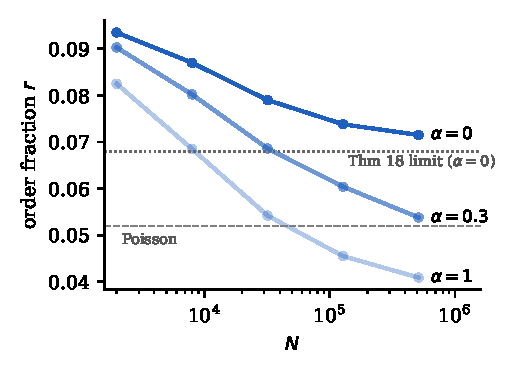
\includegraphics[width=0.62\linewidth]{figs/order_fraction.pdf}
\caption{Order fraction \(r=t(\text{2-chain})\) of the 4D
replication process along one growth path, against \(N\),
for \(\alpha=0\), \(0.3\) and \(1\); the dotted line is
uniform Poisson sprinkling. Monte Carlo error about
\(4\times10^{-4}\).}
\end{figure}

The order fraction approaches its limit slowly, as Theorem
19 predicts. For \(\alpha=0\) the decrement per doubling of
\(N\) falls from \(0.0048\) to \(0.0007\); a naive
extrapolation of these decrements gives about \(0.070\), 3\%
above the Theorem 18 value \(0.0679\), the difference being
the slowly vanishing finite-\(\tau\) correction
(\(\tau\propto N^{-1/4}\)); for \(\alpha=1\) the
extrapolated limit is about \(0.038\), while \(\alpha=0.3\)
is still pre-asymptotic at \(N=512\)k. The limit is set
entirely by the time profile: keeping the times and
redrawing the spatial positions uniformly reproduces the
order fraction (\(0.0739\) against \(0.0739\), \(0.0601\)
against \(0.0602\), \(0.0454\) against \(0.0456\)), whereas
keeping the positions and redrawing times uniformly returns
the Poisson value. Smoothing the point cloud below the
discreteness length (kernel width \(0.01\) against
\(\ell=0.044\)) changes every three-element density by at
most \(6\times10^{-4}\), equal to the Monte Carlo error,
which confirms that the limit does not see
discreteness-scale clumping. Across four realisations the
densities vary by at most \(6\times10^{-4}\), far less than
their distance to Poisson values.

The abstract measure-theoretic layer of Theorems 17--20 is
machine-checked in Lean (Sec. VIII).

\hypertarget{rogue-posets-and-the-failure-of-order-only-rules}{%
\section{Rogue posets and the failure of order-only
rules}\label{rogue-posets-and-the-failure-of-order-only-rules}}

A dynamics that works in coordinates must still be judged by
its order alone. We therefore built an intrinsic test
battery that reads only the relation matrix, and used it to
ask whether the replication rule can be replaced by a rule
that never sees coordinates.

\hypertarget{the-intrinsic-battery}{%
\subsection{The intrinsic
battery}\label{the-intrinsic-battery}}

Intervals are selected by element count, so every test is
invariant. The battery measures the Myrheim--Meyer dimension
from the order fraction \cite{Myrheim78, Meyer88}, the
midpoint dimension \(\log_2(n/n_{\rm half})\), the link
fraction, the interval-abundance spectrum \(N_k/R\) (pairs
with exactly \(k\) elements between them) \cite{GS13}, the
2D BD action per element, the height and the fraction of
minimal elements. We add one statistic that proved decisive:
the spread of the Myrheim--Meyer dimension across intervals.
Calibration shows why several tests are needed. Transitive
percolation at \(p=0.05\) fools the dimension estimator
(\(d_{\rm MM}=1.93\)) but is exposed by the abundance
spectrum, which peaks at \(k=1\)--\(2\), and by the BD
action (\(S/n=+3.43\)). KR orders fail every test. Output of
the replication model passes all of them: in 2D, deviations
from flat sprinkling range from 1\% (\(\alpha=0\)) to 5\%
(\(\alpha=3\)), and re-sprinkling with the grown density
field reproduces 60--80\% of that deviation, so most of it
is the conformal factor rather than microstructure.

In 2D the rule can be made fully intrinsic. A 2D order is
determined by its realizer, a pair of linear orders, up to
symmetry, so the realizer can serve as ordinal light-cone
coordinates. Placing the child with
\(\Delta u\,\Delta v=m\,x\), \(x\sim{\rm Exp}(1)\), and
\(\Delta u/\Delta v=e^{2\eta}\) (one element's proper
volume, uniform rapidity) passes the battery. A naive kernel
that keeps both rank displacements small instead grows
filamentary chains (\(d_{\rm MM}=1.15\)--\(1.7\)), a direct
order-theoretic image of Sec. III. The realizer trick does
not extend to 4D, because Minkowski sprinklings have no
finite realizer dimension. This is the core of the
rogue-poset problem in four dimensions.

\hypertarget{three-families-of-order-only-insertion-three-failures}{%
\subsection{Three families of order-only insertion, three
failures}\label{three-families-of-order-only-insertion-three-failures}}

An order-only insertion chooses a down-set \(D\) and an
up-set \(U\) with every element of \(D\) below every element
of \(U\), and makes the new element the cut between them.
Its past and future cannot be inferred from each other. We
tested every natural way of choosing them; each family fails
in a characteristic way.

\begin{longtable}[]{@{}
  >{\raggedright\arraybackslash}p{(\columnwidth - 6\tabcolsep) * \real{0.1167}}
  >{\raggedright\arraybackslash}p{(\columnwidth - 6\tabcolsep) * \real{0.3333}}
  >{\raggedright\arraybackslash}p{(\columnwidth - 6\tabcolsep) * \real{0.3833}}
  >{\raggedright\arraybackslash}p{(\columnwidth - 6\tabcolsep) * \real{0.1667}}@{}}
\toprule\noalign{}
\begin{minipage}[b]{\linewidth}\raggedright
Family
\end{minipage} & \begin{minipage}[b]{\linewidth}\raggedright
Representative rule
\end{minipage} & \begin{minipage}[b]{\linewidth}\raggedright
2D outcome (\(N=2000\); sprinkling: \(d_{\rm MM}=2.00\),
link fraction \(0.07\))
\end{minipage} & \begin{minipage}[b]{\linewidth}\raggedright
Failure
\end{minipage} \\
\midrule\noalign{}
\endhead
\bottomrule\noalign{}
\endlastfoot
Closure & Galois closure: future \(=\) all upper bounds of
the chosen past & Height \(510\)--\(617\) against \(79\);
\(d_{\rm MM}=1.30\)--\(1.37\); \(S/n\approx1.00\) & Too many
relations; positive feedback grows chains \\
Minimal cuts & Past \(=J^-[x]\), future \(=J^+[b]\) for a
small interval \(I(x,b)\) & \(d_{\rm MM}=2.9\)--\(3.2\) &
Too few relations \\
Link-level mutation & Clone a parent, drop links with
probability \(\mu\), add siblings with probability
\(\gamma\) & Mean quantities tunable to a few per cent;
spread of \(d_{\rm MM}\) across intervals \(0.20\)--\(0.28\)
against \(0.05\); 2--3\% exact twins & Fluctuations;
parameters not portable between dimensions \\
Element-level moves & Clone, then single-element boundary
moves to a volume-controlled displacement &
\(d_{\rm MM}=2.5\)--\(3.9\); link fraction
\(0.26\)--\(0.62\) & Light cones become jagged \\
\end{longtable}

The closure failure persists even with an oracle. If the new
element receives its true geometric past and only its future
comes from the closure, spurious relations per insertion
grow from a median of \(3\) early to \(17\) late, and the
height grows from \(79\) to \(191\). The bias is one-sided,
because the true future is always contained in the closure,
so it accumulates. In static 4D sprinklings the closure adds
about \(0.3\) spurious relations per past link, growing as
roughly \(\sqrt N\) (26, 50 and 99 at \(N=2\)k, 8k, 32k),
whereas in 2D it stays near 2.

The jagged-cone failure is structural, not a matter of
counts. Forcing the relation count to be conserved leaves
the outcome unchanged; every boundary move links the new
element to some arbitrary boundary element, so the cone
loses coherence. Larger displacements make it worse: at
three times the nearest-neighbour displacement the link
fraction is eight times the sprinkled value.

\hypertarget{the-mechanism-order-space-neighbours-are-far-apart}{%
\subsection{The mechanism: order-space neighbours are far
apart}\label{the-mechanism-order-space-neighbours-are-far-apart}}

All three failures have one cause. Define the order distance
\(\Delta(c,y)\) as the number of elements related
differently to \(c\) and to \(y\). In a sprinkling, the
median distance to the order-nearest neighbour is \(18\),
\(26\), \(38\) at \(N=1\)k, 2k, 4k in 2D, about
\(0.59\sqrt N\), and \(20\), \(38\), \(68\) in 4D, about
\(N^{0.8}\). The thin shell between the light cones of two
nearby points extends along null directions to the boundary
of the region, so no displacement of \(O(1)\) elements
exists. A rule that edits relations locally cannot move a
light cone coherently. A geometric displacement does exactly
that, which is why the successful rules (the 2D realizer
rule and the coordinate model) carry structure beyond the
order. The same geometric fact underlies the growth of
closure errors and the non-amenability noted in Sec. III.

We conclude that the coordinate model is the dynamics, while
the intrinsic battery and the poset-limit theorems are
verification tools. The answer to the rogue-poset problem
offered here is that the coordinate model's output passes
every intrinsic test, and that order-only local rules
necessarily produce jagged or rogue structure. Section VII
asks whether quantum interference can remove that structure
after the fact.

\hypertarget{quantum-dynamics-interference-and-the-defect-gas}{%
\section{Quantum dynamics: interference and the defect
gas}\label{quantum-dynamics-interference-and-the-defect-gas}}

Section VI leaves a precise question. Order-only growth
rules produce non-manifold structure of specific kinds:
near-chains from closure, jagged cones from element moves,
clone families from mutation. Attaching the phase
\(e^{i\beta S_{\rm BD}}\) to the histories of such a rule,
does interference remove the non-manifold branches?

\hypertarget{phases-on-a-growth-tree-telescope}{%
\subsection{Phases on a growth tree
telescope}\label{phases-on-a-growth-tree-telescope}}

We follow the path-sum convention in which the amplitude of
an event is the coherent sum over its members
\cite{Surya12, LC18, CCS23}, within Sorkin's
quantum-measure framework \cite{Sorkin94}. If every growth
step carries the phase \(e^{i\beta\Delta S}\), the phase of
a history is \(e^{i\beta(S(C_N)-S(C_1))}\), so all histories
ending in the same poset are in phase. The growth tree only
supplies weights \(w(C)=\sum_h\sqrt{p(h)}\), and
interference happens only between different final posets. A
decoherence functional that is diagonal in final posets
would make the phase irrelevant altogether.

A class \(\Gamma\) of posets is not suppressed merely
because its measure falls below its \(\beta=0\) value:
random phases already reduce every class to the ``random
floor'' \(\sqrt{\sum w^2}\), which favours small classes
relative to large ones. The right diagnostic is the excess
cancellation

\[E_\Gamma(\beta)=\frac{\left|\sum_{C\in\Gamma}w(C)\,e^{i\beta S(C)}\right|^2}{\sum_{C\in\Gamma}w(C)^2},\]

equal to 1 for random phases, below 1 for systematic
cancellation and above 1 for partial coherence.

\hypertarget{exact-enumeration-and-variance-scaling}{%
\subsection{Exact enumeration and variance
scaling}\label{exact-enumeration-and-variance-scaling}}

Enumerating all posets with \(N\le8\) (matching OEIS A000112
and A001035), the geometric mean of \(E_\Gamma\) over
\(\beta\in(0,\pi]\) for the 2D action is \(0.09\), \(0.03\),
\(0.01\) at \(N=6,7,8\) for two-layer posets: they cancel
systematically, increasingly with \(N\), reproducing at
small \(N\) the Loomis--Carlip mechanism \cite{LC18}.
Three-layer (KR-type) posets sit at the random level
(\(0.88\)--\(1.30\)), as expected at sizes far from the
asymptotic regime of \cite{CCS23}. 2D orders are partially
coherent (\(1.42\), \(3.20\), \(6.27\)), because their
actions are relatively concentrated.

For \(N=50\)--\(400\) we sample each class 300 times and
measure the scaling of \({\rm Var}(S)\). With the unsmeared
2D action, sprinkled causal sets have
\({\rm Var}\propto N^{1.42}\), clone families \(N^{1.59}\),
KR orders \(N^{2.04}\) and jagged-cone orders \(N^{3.11}\);
near-chains from closure have a variance a thousand times
smaller than sprinkling, because an \(n\)-chain has
\(S_2=n\) exactly. Smearing (\(\epsilon=0.1\)) removes this
spurious coherence of near-chains (their variance rises to
\(2.1\) times the sprinkled value) and also tames the large
fluctuations of the unsmeared 4D action on sprinklings
(exponent \(2.27\) at \(\epsilon=1\), \(1.84\) at
\(\epsilon=0.03\)).

Variance alone cannot decide suppression. In the Gaussian
approximation the coherent part of a class amplitude is
\(W\,e^{-\beta^2{\rm Var}/2}\); once this falls below the
random floor \(\sqrt W\), the amplitude is
\(|A_\Gamma|^2=E_\Gamma W\). A class of entropy \(W\) can
therefore be pushed only to \(\sqrt W\) by large variance,
and for KR orders \(\sqrt W=2^{N^2/8}\) still dwarfs the
\(e^{O(N\log N)}\) entropy of manifoldlike classes. Beating
entropy requires structural cancellation, \(E_\Gamma\ll1\).

\hypertarget{the-kr-threshold-as-a-lock-window}{%
\subsection{The KR threshold as a lock
window}\label{the-kr-threshold-as-a-lock-window}}

KR orders supply the cleanest example of structural
cancellation. With \(\epsilon=1\) their 4D action is
\(S_4\approx(4/\sqrt6)(N-N_0)\), where the link count
\(N_0\) is binomial with \(M=N^2/4\) trials and \(p=1/2\)
(measured \({\rm Var}(S_4)/N^2=0.164\) against the predicted
\((16/6)\,{\rm Var}(N_0)/N^2=(8/3)(1/16)=1/6\)). The sum
over link configurations is then an exact product,

\[|A_{\rm KR}|=\left|2\cos(\beta'/2)\right|^{M},\qquad \beta'=\frac{4}{\sqrt6}\,\beta ,\]

which falls below the amplitude of a single configuration
iff \(\beta'\in(2\pi/3,4\pi/3)\), i.e.~\(\beta>1.2825\).
With \(\beta=(\ell/\ell_p)^2\) the threshold is
\(\ell>1.1325\,\ell_p\), within \(0.3\%\) of the bound
\(\ell\gtrsim1.136\,\ell_p\) obtained by Carlip, Carlip and
Surya for \(d=4\) \cite{CCS23, Carlip24}. The suppression
is a window, repeating every \(2\pi\) in \(\beta'\), rather
than a monotone effect. The mechanism is phase locking:
every ``site'' (a potential link) shifts the action by the
same amount.

\hypertarget{the-defect-gas-theorem}{%
\subsection{The defect-gas
theorem}\label{the-defect-gas-theorem}}

The non-manifold structure of Sec. VI is not of this kind.
It consists of local defects of several types (twins, jagged
clones, mutated clones, cut links) whose action shifts are
widely spread. We model it as a defect gas.

\textbf{Theorem 21 (defect gas).} Let a background \(C_0\)
carry \(M\) sites, each with options \(j\in\{0,1,\dots,K\}\)
(\(j=0\) clean), such that every combination is a distinct
causal set and the action is additive,
\(S=S_0+\sum_s\delta(s,j_s)\). Then

\[\sum_{\rm configurations}e^{i\beta S}=e^{i\beta S_0}\prod_{s=1}^MP(s,\beta),\qquad P(s,\beta)=\sum_{j=0}^Ke^{i\beta\delta(s,j)},\]

so the growth rate relative to the clean configuration is
exactly
\(r_M(\beta)=M^{-1}\sum_s\ln\left|1+\sum_{j\ge1}e^{i\theta_{s,j}}\right|\)
with \(\theta_{s,j}=\beta(\delta(s,j)-\delta(s,0))\). If the
phase vectors \(\theta_s\in\mathbb T^K\) are pairwise
independent and uniformly distributed, then almost surely
the sum is nonzero for every \(M\) and

\[r_M(\beta)\longrightarrow m(1+x_1+\dots+x_K)=\int_{\mathbb T^K}\ln\left|1+e^{i\theta_1}+\dots+e^{i\theta_K}\right|\,d\theta ,\]

the Mahler measure \cite{Mahler62}. Moreover \(m(1+x)=0\)
and \(m(1+x_1+\dots+x_K)>0\) for \(K\ge2\).

\emph{Proof.} (i) The factorisation is the finite identity
``sum of products equals product of sums'' together with
\(e^{\sum}=\prod e\); the common factor
\(e^{i\beta\delta(s,0)}\) has modulus one. (ii) The rate is
the empirical mean of \(\ln|W_K(\theta_s)|\) with
\(W_K(\theta)=1+\sum_je^{i\theta_j}\). Integrating out one
phase with Jensen's formula,
\(\int\ln|e^{it}+w|\,dt/2\pi=\log^+|w|\), and using the
uniform bound \(\int|\ln|e^{it}+w||\,dt/2\pi\le2\ln(1+|w|)\)
with Tonelli's theorem, \(\ln|W_K|\) is integrable and the
strong law of large numbers gives the limit. (iii) The same
inner Jensen step gives
\(m(1+x_1+\dots+x_K)=\mathbb E\,\log^+|1+x_2+\dots+x_K|\),
which is \(\log^+1=0\) for \(K=1\). For \(K\ge2\) it is
positive, because on the box \(\theta_j\in(0,\pi/2)\), of
measure \(4^{-(K-1)}\), the real part of \(1+x_2+\dots+x_K\)
exceeds 1. (iv) On each slice, \(e^{it}=c\) has at most one
solution in \((0,2\pi]\), so the zero set of \(W_K\) is
null. \(\square\)

The values are
\(m(1+x+y)=(3\sqrt3/4\pi)L(\chi_{-3},2)=0.3231\) and
\(m(1+x+y+z)=7\zeta(3)/2\pi^2=0.4263\) \cite{Smyth81}, and
numerically \(m=0.5444\) for \(K=4\); for large \(K\),
\(m\approx\tfrac12\ln K\). The classical entropy per site is
\(\ln(K+1)\), so interference removes roughly half of it,
the analytic form of the random floor of Sec. VII B.
Suppression below the clean configuration (\(r<0\)) requires
phases far from uniform. For a single shift \(\delta\),
\(|1+e^{i\beta\delta}|<1\) iff \(\cos\beta\delta<-1/2\): all
sites must sit in the lock window simultaneously, which is
the KR situation of Sec. VII C. Every step of the proof,
including the integrability, the Fubini step, the null zero
set and the strong-law substitution, is checked in Lean
(Sec. VIII); uniformity of the phases is an explicit
hypothesis there.

\hypertarget{tests-of-the-hypotheses}{%
\subsection{Tests of the
hypotheses}\label{tests-of-the-hypotheses}}

\textbf{Shifts and additivity.} On 2D sprinkled diamonds
(\(N=300\), every site) the single-defect shifts are broad:
for the unsmeared action their standard deviation is
\(25\)--\(44\) (cuts smallest), for \(\epsilon=0.1\) it is
\(0.06\)--\(0.20\). In 4D they are broader still. Five
far-apart twins shift the action by \(-370\) against a sum
of singles of \(-366\); five far-apart cuts give \(-40\)
against \(-40\).

\textbf{Uniformity of the phases.} For integer-valued shifts
the phases are periodic in \(\beta\) (period \(\pi\) for the
unsmeared 2D action, whose shifts are even), so we scan one
period and compare the empirical rate with the Mahler value.

\begin{figure}
\centering
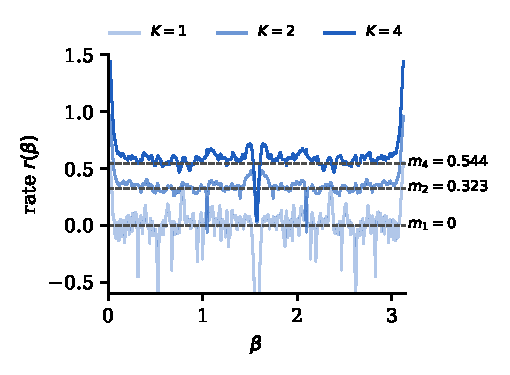
\includegraphics[width=0.62\linewidth]{figs/rate_beta.pdf}
\caption{Empirical defect-gas rate
\(r(\beta)=M^{-1}\sum_s\ln|1+\sum_{j\le K}e^{i\beta\delta_{s,j}}|\)
over \(M=300\) sites of a 2D sprinkled diamond (unsmeared
action), for one defect type (\(K=1\), twins), two (\(K=2\),
twins and cuts) and four. Dashed lines: Mahler measures.
Dips mark lattice resonances of the integer-valued action.}
\end{figure}

\begin{longtable}[]{@{}
  >{\raggedright\arraybackslash}p{(\columnwidth - 8\tabcolsep) * \real{0.1667}}
  >{\raggedright\arraybackslash}p{(\columnwidth - 8\tabcolsep) * \real{0.2833}}
  >{\raggedright\arraybackslash}p{(\columnwidth - 8\tabcolsep) * \real{0.2333}}
  >{\raggedright\arraybackslash}p{(\columnwidth - 8\tabcolsep) * \real{0.1333}}
  >{\raggedright\arraybackslash}p{(\columnwidth - 8\tabcolsep) * \real{0.1833}}@{}}
\toprule\noalign{}
\begin{minipage}[b]{\linewidth}\raggedright
Setting
\end{minipage} & \begin{minipage}[b]{\linewidth}\raggedright
Phase non-uniformity, median over \(\beta\) (uniform
\(\approx0.058\))
\end{minipage} & \begin{minipage}[b]{\linewidth}\raggedright
\(K=2\): rate at generic \(\beta\) (Mahler \(0.323\))
\end{minipage} & \begin{minipage}[b]{\linewidth}\raggedright
\(K=2\): fraction of \(\beta\) with \(r<0\)
\end{minipage} & \begin{minipage}[b]{\linewidth}\raggedright
\(K=4\): minimum rate over \(\beta\) (Mahler \(0.544\))
\end{minipage} \\
\midrule\noalign{}
\endhead
\bottomrule\noalign{}
\endlastfoot
2D, \(\epsilon=1\) & \(0.050\)--\(0.066\) &
\(0.336\pm0.045\) & \(0.5\%\) & \(+0.042\) \\
2D, \(\epsilon=0.1\) & \(0.55\)--\(0.94\) &
\(0.318\pm0.041\) & \(0\) & \(+0.459\) \\
4D, \(\epsilon=1\) & \(0.048\)--\(0.058\); cuts \(0.46\) &
(cuts never generic) & \(0.5\%\) & \(+0.239\) \\
4D, \(\epsilon=0.1\) & \(0.11\)--\(0.93\) & (never generic)
& \(0\) & \(+0.346\) \\
\end{longtable}

Non-uniformity is the median over \(\beta\) of
\(|\langle e^{i\beta\delta}\rangle|\) across the four defect
types; ``generic'' \(\beta\) are those where every involved
type is within three times the uniform level. For the
unsmeared 2D action the phases are as uniform as 300 sites
allow at 88\% of \(\beta\), and the rate there matches
Mahler for \(K=2\) (\(0.336\) against \(0.323\)) and \(K=4\)
(\(0.585\) against \(0.544\)). For one type the
\(\beta\)-average is \(+0.014\), consistent with Jensen's
zero, with sign changes across \(\beta\). Where uniformity
fails, as for small smeared shifts at moderate \(\beta\) or
for 4D cuts, the phases bunch near zero and the rate rises
above the Mahler value. Suppression (\(r<0\)) occurs only in
narrow lattice resonances, on \(0.5\%\) of \(\beta\) for
\(K=2\) and never for \(K=4\).

\textbf{Overlap and interaction.} Overlapping or causally
related defects are not additive. We built every
configuration explicitly (cuts first, then twins copying the
cut relations, twin--twin relations following their sites)
on \(N=200\) sprinkled diamonds and summed the phases
exactly, for dilute sites (farthest-point sampling) and
dense sites (nearest to the centre), averaged over three
backgrounds.

\begin{longtable}[]{@{}
  >{\raggedright\arraybackslash}p{(\columnwidth - 6\tabcolsep) * \real{0.2333}}
  >{\raggedright\arraybackslash}p{(\columnwidth - 6\tabcolsep) * \real{0.2500}}
  >{\raggedright\arraybackslash}p{(\columnwidth - 6\tabcolsep) * \real{0.2500}}
  >{\raggedright\arraybackslash}p{(\columnwidth - 6\tabcolsep) * \real{0.2667}}@{}}
\toprule\noalign{}
\begin{minipage}[b]{\linewidth}\raggedright
Sites, defect types
\end{minipage} & \begin{minipage}[b]{\linewidth}\raggedright
\(M=4\)
\end{minipage} & \begin{minipage}[b]{\linewidth}\raggedright
\(M=8\)
\end{minipage} & \begin{minipage}[b]{\linewidth}\raggedright
\(M=12\)
\end{minipage} \\
\midrule\noalign{}
\endhead
\bottomrule\noalign{}
\endlastfoot
Dense, \(K=1\) (twins) & \(0.214\pm0.042\) / \(0.006\) &
\(0.265\pm0.011\) / \(0.004\) & \(0.306\pm0.006\) /
\(0.001\) \\
Dilute, \(K=1\) & \(0.076\pm0.059\) / \(0.015\) &
\(0.127\pm0.056\) / \(0.008\) & \(0.137\pm0.032\) /
\(0.006\) \\
Dense, \(K=2\) (twins, cuts) & \(0.437\pm0.020\) / \(0.327\)
& \(0.477\pm0.022\) / \(0.358\) & \(0.515\pm0.006\) /
\(0.346\) \\
Dilute, \(K=2\) & \(0.411\pm0.048\) / \(0.385\) &
\(0.383\pm0.029\) / \(0.317\) & \(0.424\pm0.036\) /
\(0.340\) \\
\end{longtable}

Each cell gives the \(\beta\)-averaged rate from the exact
configuration sum (mean \(\pm\) standard error over three
backgrounds) and, after the slash, the product formula of
Theorem 21 built from the single-defect shifts. The exact
rate exceeds the product formula at every \(M\) and in every
setting, and the excess does not shrink as \(M\) grows. For
dense twins the exact rate reaches \(0.317\pm0.006\) at
\(M=16\) while the product (Jensen) value stays at zero; for
dense two-type defects the excess is \(0.10\)--\(0.17\). At
individual \(\beta\) the exact rate is higher on 66--92\% of
the scan, and the fraction of \(\beta\) with a negative
exact rate falls with \(M\) (dense, \(K=2\): from \(2.9\%\)
at \(M=4\) to zero for \(M\ge10\)). Because the background
is fixed (\(N=200\)), larger \(M\) also means more closely
spaced sites, so the \(M\)-dependence mixes system size with
defect density. The robust conclusion is that interactions
act like additional phase randomness and raise the rate.

\textbf{No double counting.} The path sum counts each
unlabelled causal set once, so distinct configurations must
give non-isomorphic posets. For \(M=8\), \(K=2\), two
backgrounds and both site sets, all \(3^8=6561\)
configurations receive distinct Weisfeiler--Lehman
invariants (refinement over past and future colour
multisets). Distinct invariants imply non-isomorphism, so no
configuration is counted twice. At \(N=8\), where every
poset can be enumerated, the non-2D orders produced by the
classical rules sit at the random level,
\(E=0.86\)--\(1.23\), as the theorem predicts.

\hypertarget{conclusion-of-the-quantum-test}{%
\subsection{Conclusion of the quantum
test}\label{conclusion-of-the-quantum-test}}

Interference on a classical growth tree does not remove the
multi-type local defects generated by order-only rules:
their amplitude grows at the Mahler rate, about half the
classical entropy rate, and interactions between defects
raise it further. Interference does remove classes whose
action shifts phase-lock, and the KR threshold is the clean
instance. Whether a class is suppressed is thus a computable
property of its shift distribution, not of its variance.

\hypertarget{formal-verification-in-lean-4}{%
\section{Formal verification in Lean
4}\label{formal-verification-in-lean-4}}

We used Lean 4 \cite{Lean4} with Mathlib \cite{Mathlib20}
as a check on the proofs, not as a substitute for them. Five
files compile without \texttt{sorry}; every theorem depends
only on the standard axioms \texttt{propext},
\texttt{Classical.choice} and \texttt{Quot.sound}. The
toolchain is Lean 4.36.0-rc1 with Mathlib built from source;
all declarations live in the namespace
\texttt{CausalDensification}.

\begin{longtable}[]{@{}
  >{\raggedright\arraybackslash}p{(\columnwidth - 4\tabcolsep) * \real{0.3667}}
  >{\raggedright\arraybackslash}p{(\columnwidth - 4\tabcolsep) * \real{0.5500}}
  >{\raggedright\arraybackslash}p{(\columnwidth - 4\tabcolsep) * \real{0.0833}}@{}}
\toprule\noalign{}
\begin{minipage}[b]{\linewidth}\raggedright
File
\end{minipage} & \begin{minipage}[b]{\linewidth}\raggedright
What is verified
\end{minipage} & \begin{minipage}[b]{\linewidth}\raggedright
Theorems
\end{minipage} \\
\midrule\noalign{}
\endhead
\bottomrule\noalign{}
\endlastfoot
\texttt{UndampedKernelConstants.lean} & Theorem 18
constants: bounds on \(Z(t)\), \(\int_0^T|x-t|\,dx=Z(t)\),
stationarity \(\int Z(t)q(x|t)\,dt=Z(x)\), \(\int Z=1/24\),
\(T/Z\le8\); Lipschitz constant 80 of \(q\); bounds on the
shell-overlap length \(\ell\); \(h_{abc}\ge0.035\); the
Doeblin constant; the L2 constants \(288\), \(20\) and
\(436\) & 19 \\
\texttt{PosetLimitCore.lean} & Theorem 17 for pairs on
\(\mathbb R\times\mathbb R^3\) (product-measure continuity,
portmanteau, boundary of the causal relation contained in
null pairs); summability for Theorem 19; for Theorem 20 the
Pólya identities, the exact same-class probability
\(2(N-M)/((M+1)(N-1))\le2/(M+1)\), the shell volume bound,
the Jacobian cancellation and the choice
\(M=\lceil\varepsilon^{-1/2}\rceil\) & 14 \\
\texttt{PosetLimitFramework.lean} & Theorem 17 for general
\(k\) and on slab \(\times\,\mathbb T^3\) with minimum-image
distance; the Fatou step of Theorem 20; summable second
moments imply a.s. convergence; Doeblin implies uniform
geometric ergodicity; bounded martingale differences plus
summable drift imply a.s. convergence; the telescoping
identity of Theorem 18 & 28 \\
\texttt{DefectGasAlgebra.lean} & Theorem 21: exact
factorisation; Jensen's formula for \(1+x\); the inner
Jensen identity; the lock window & 4 \\
\texttt{DefectGasLimit.lean} & Theorem 21: integrability and
the Fubini step on the torus,
\(m(1+x_1+\dots+x_K)=\int_{\mathbb T^{K-1}}\log^+|1+x_2+\dots+x_K|\)
(the Lean statement indexes the \(K\) phases from 0);
\(m=0\) for \(K=1\) and \(m>0\) for \(K\ge2\); the zero set
is null; the strong-law substitution; the full statement of
Theorem 21 & 24 \\
\end{longtable}

The checks found two errors, both in bookkeeping rather than
in mathematics. A Pólya same-class probability had been
written with an \(O(1/N)\) correction that does not exist;
the exact finite-\(N\) formula has none. And a summation
index in the \(L^1\) bound of Theorem 19 had been typed so
that Lean read it as a real number, for which the series is
defined to be zero; with a natural-number index the proof
goes through.

Two layers remain unformalised. The first consists of
analysis tools missing from Mathlib: the three-shell
convolution formula and the \(W^{1,1}\) translation estimate
\({\rm TV}(\mu,\mu_e)\le\tfrac12|e|\,\|\nabla p\|_1\). The
second is modelling: writing the replication process as a
stochastic process in Lean and verifying the hypotheses of
the abstract theorems (the minorisation of \(K^5\),
stationarity, the perturbation bound L3, autonomy of the
time process). In Theorem 21 the uniform-phase hypothesis is
an explicit assumption of the Lean statement, not a theorem.

\hypertarget{discussion-and-open-problems}{%
\section{Discussion and open
problems}\label{discussion-and-open-problems}}

The replication model answers the four problems in different
currencies. The continuum limit is proved: for every damping
the process has a poset limit, a uniform sprinkling of a
conformally flat spacetime, and below the damping length the
grown set satisfies high-probability, uniform versions of
Madsen's F2 and F3 for the conformal metric. Lorentz
invariance at the discreteness scale is established
numerically to a few per cent, with violation confined to
the clumping excess. The rogue-poset problem is answered by
verification rather than by an order-intrinsic dynamics: the
model's output passes every intrinsic test, and three
families of order-only rules fail for a single geometric
reason. On quantum dynamics the result is negative but
precise. Phase interference suppresses a class only when its
action shifts phase-lock, as for layered and KR orders.
Multi-type local defects grow at the Mahler rate, and
interactions between overlapping defects make them grow
faster.

The negative result fits the positive ones. Section VI shows
that order-only local rules generate jagged, multi-type
defects; Section VII shows that \(e^{i\beta S_{\rm BD}}\)
cannot remove them. A viable dynamics must therefore carry
coherent light-cone structure from the start, as the
coordinate model does. Interference is still useful: it
removes the entropically dominant layered orders that no
classical rule would want to produce in the first place.

Several problems remain open.

\begin{enumerate}
\def\labelenumi{\arabic{enumi}.}
\tightlist
\item
  \textbf{An order-intrinsic 4D dynamics.} The most
  promising route we see uses the link-level mutation of
  Sec. VI B as a proposal and the local BD action or the
  abundance spectrum as a Metropolis acceptance, letting the
  action select coherent light cones.
\item
  \textbf{The uniform-phase hypothesis.} For the unsmeared
  action the shifts are integers, so uniformity at generic
  \(\beta\) should follow from an equidistribution argument
  once the shift distribution is controlled. Smeared actions
  need a separate treatment, although there the failure of
  uniformity only raises the rate.
\item
  \textbf{The large-scale conformal factor.} Replication
  fixes it by boundary conditions. Whether the Lorentzian
  path sum selects an expanding FRW profile on replicated
  sets is untested.
\item
  \textbf{Sharper constants.} Theorem 8 is about 2.7 times
  looser than the measured supremum; the F3 bounds stop at
  the Talagrand \(\sqrt L\) scale, while true fluctuations
  are smaller \cite{BDJ99, BL15}; and the law of the random
  limit profile for \(\alpha>0\) is unknown.
\item
  \textbf{The Lean instantiation layer} (Sec. VIII).
\end{enumerate}

All simulations use the scripts of the accompanying research
log (Python with NumPy; a C program for chain heights), and
the five Lean files are available with it.


\bibliographystyle{\ifdefined\usingrevtex apsrev4-2\else unsrtnat\fi}
\bibliography{refs}

\end{document}
